\documentclass[10pt,a4paper,titlepage]{article}
\usepackage[utf8]{inputenc}
\usepackage{amsmath}
\usepackage{amsfonts}
\usepackage{amssymb}
\usepackage{makeidx}
\usepackage{enumitem}
\usepackage{graphicx}
\usepackage{longtable}
\usepackage[hidelinks]{hyperref}

%this is a command used in the title template
\newcommand{\HRule}{\rule{\linewidth}{0.5mm}}

%questo fa in modo che le liste numerate siano allineate come le altre
\setenumerate{leftmargin=*, labelindent=\parindent}

%questo genera il toc, ricorda di eseguire due volte
\makeindex

\begin{document}
\begin{titlepage}
\begin{center}

%logo

\includegraphics[width=0.30\textwidth]{./images/logo}~\\[1cm]
\textsc{\LARGE Politecnico di Milano}\\[1.5cm]

\textsc{\Large Software Engineering 2 Project}\\[0.5cm]

% Title
\HRule \\[0.4cm]
{ \Huge \bfseries MeteoCal \\[0.4cm] }
{ \huge \bfseries Design Document \\[0.4cm] }
\HRule \\[1.5cm]

% Author
\begin{flushright}
\noindent
\large
\emph{Authors:}\\
Andrea \textsc{Celli}\\
Stefano \textsc{Cereda}
\end{flushright}
\vfill

% Bottom of the page
{\large \today}

\end{center}
\end{titlepage}

\tableofcontents

\pagebreak
\part{System Description}
MeteoCal is a web based platform. Thus users need internet access and a web browser to use the platform.

Users can navigate through the system using usual commands such as links, buttons, input forms and so on.

With a standard deploy on a local machine the web address to have access to MeteoCal is \url{http://localhost:8080/MeteoCal/login.xhtml}

\part{Unlogged User}

\section{Login}
Users can perform the login filling the two input forms. If the login is successful the user is redirected to his homepage. Otherwise an error message is shown.

From the login page an unlogged user can access registration page and about page. In order to do so he has to click on of the two links under the login button.

\begin{center}
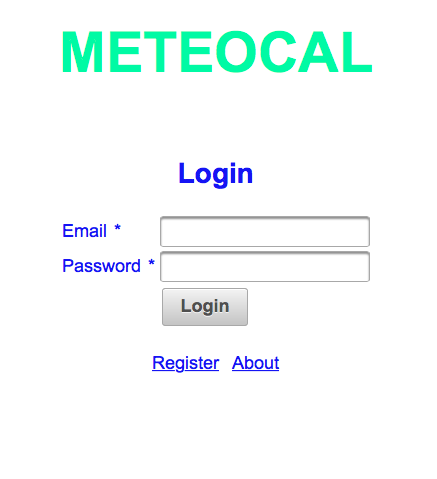
\includegraphics[width=0.7\linewidth]{./images/01_login.png}
\end{center}

\section{Register}
Users can sign-up for MeteoCal using the registration page. All the input fields are mandatory. If the registration is successful the user is redirected to the login page. Otherwise adequate error messages are shown.

From the registration page users can go back to the login or go to the about page using the links.

\begin{center}
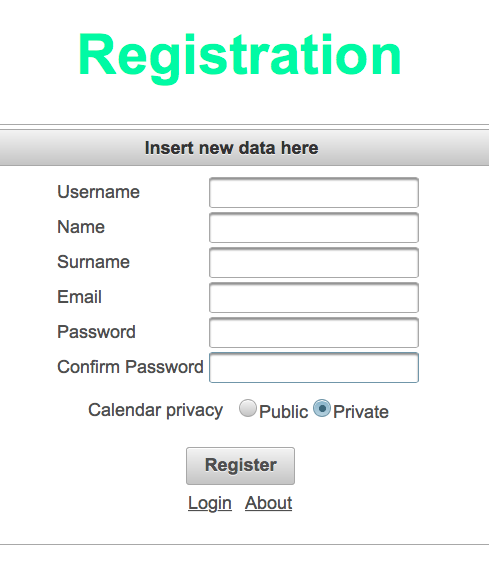
\includegraphics[width=0.7\linewidth]{./images/02_registration.png}
\end{center}

\section{View About}
Users that want more information before signing up for MeteoCal can read the About page.

The “login” and “register” links enable the user to reach the other pages available when the user is not logged.

\begin{center}
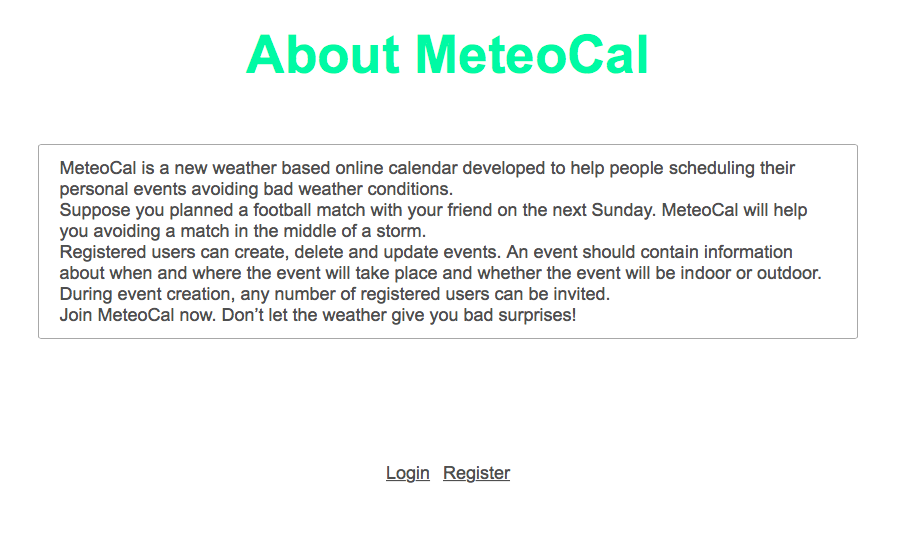
\includegraphics[width=\linewidth]{./images/03_about.png}
\end{center}

\part{Logged User}

\section{Overview}
When the user performs the login he/she is taken to the homepage.
The home contains the core of the platform: the calendar. 
These are two views of the homepage: one without any event and a quite busy one.

\begin{center}
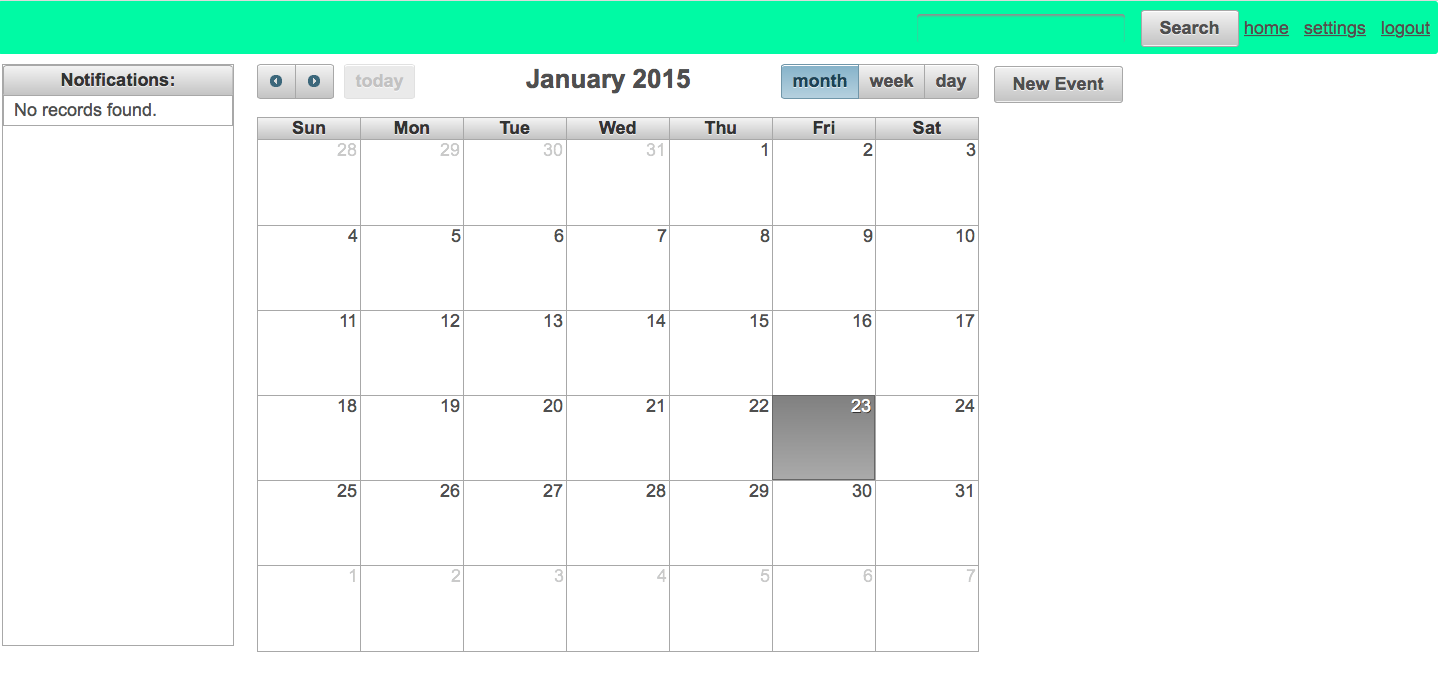
\includegraphics[width=\linewidth]{./images/04_calendar_empty.png}
\end{center}

\begin{center}
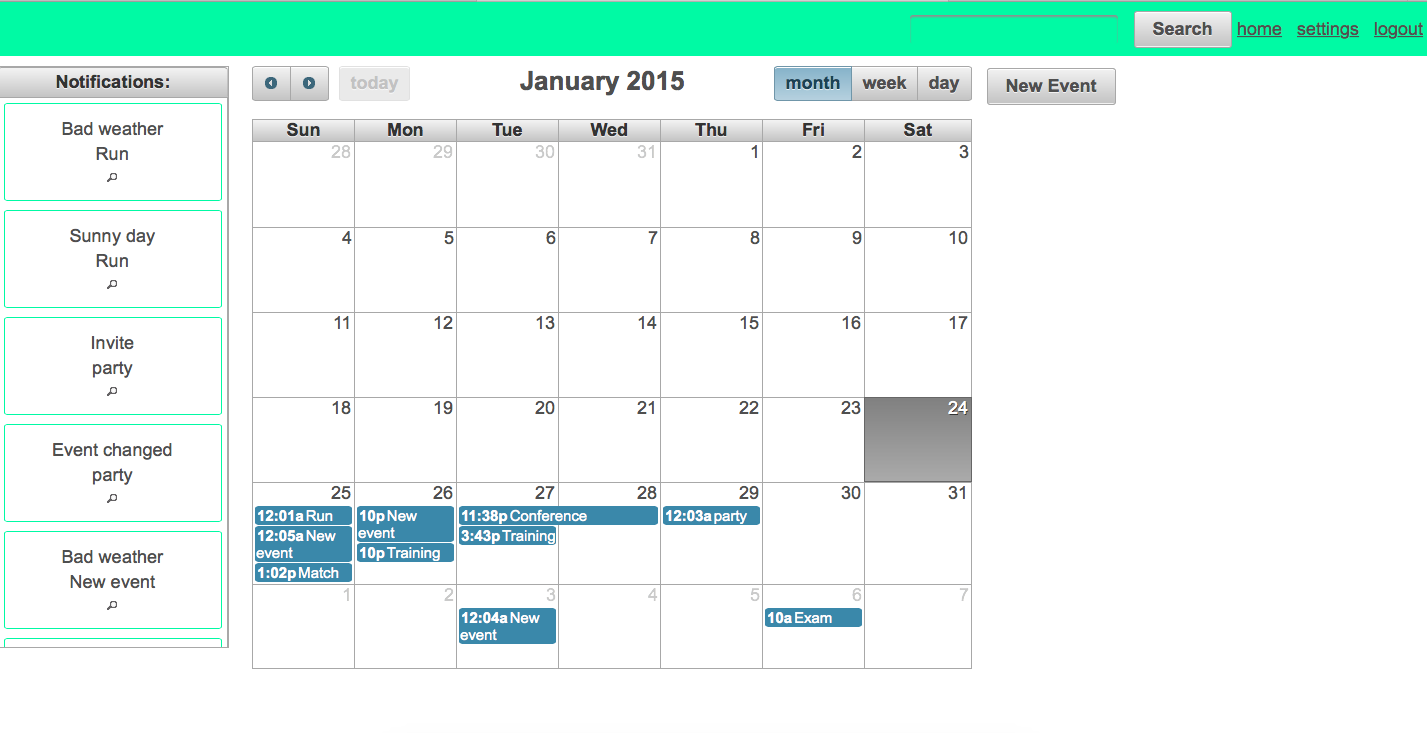
\includegraphics[width=\linewidth]{./images/05_calendar_busy.png}
\end{center}

The following schema highlights the key components of the homepage.

\begin{center}
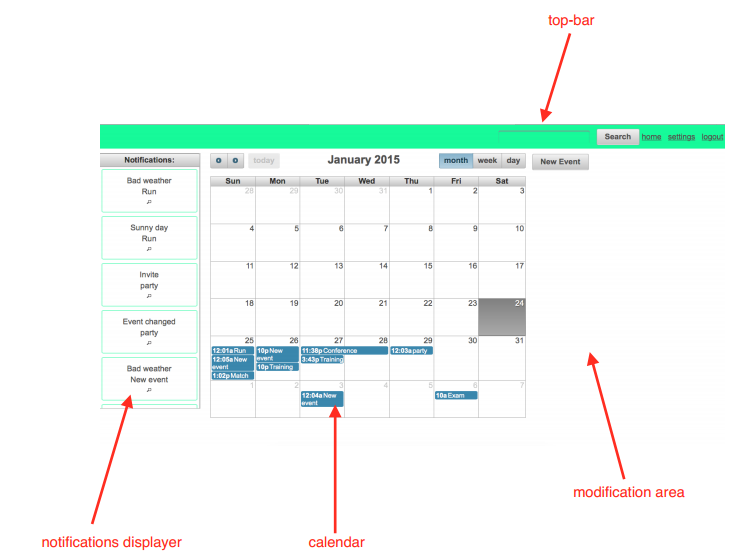
\includegraphics[width=\linewidth]{./images/06_home_arrows}
\end{center}

The top-bar is displayed in every page available for the logged user. It allows to search another user by writing the search key in the input form and clicking on the search button. 

Moreover users can reach their settings page, go back to their home or logout.

\begin{center}
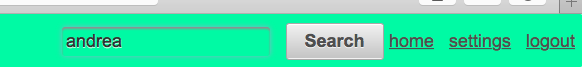
\includegraphics[width=\linewidth]{./images/07_search_bar.png}
\end{center}

\section{Manage Calendar}

\subsection{Browse Calendar}
Users can browse their calendar using the commands placed at the top left of it. They can also choose between different type of view using the buttons on the top right of the calendar.

\begin{center}
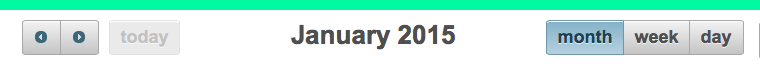
\includegraphics[width=\linewidth]{./images/08_calendar_top.png}
\end{center}

\subsection{Create event}
If you want to create a new Event you have to click on the New Event button, placed on the right of the calendar.
After clicking on the New Event button the following dialog appears on the right of the calendar.
Using this dialog you can specify all the event details. None of the details is mandatory. 

If the title is not specified it’s set to “new event” by default. If the start/end of the event are not specified they’re set to the current time by default. 

You can save or reset the event using the related buttons. If you close the dialog without saving nothing happens.

\begin{center}
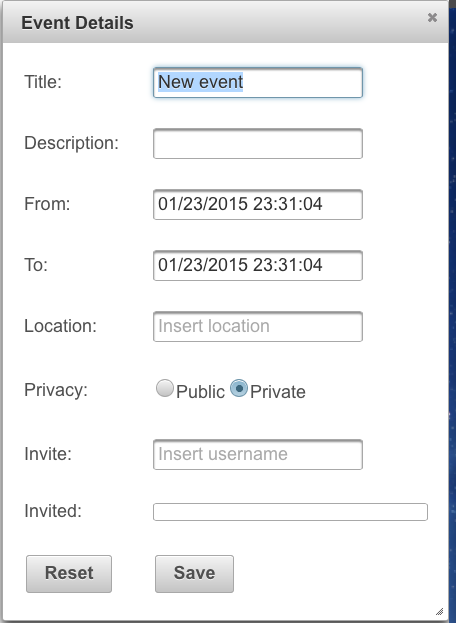
\includegraphics[width=0.7\linewidth]{./images/09_create_event.png}
\end{center}

You can select dates typing into the form or using the calendar.
Neither starting time in the past nor ending time before the start will be allowed.

From the picture you can see the calendar to select the end date. Note that dates before the start 
are not selectable.

\begin{center}
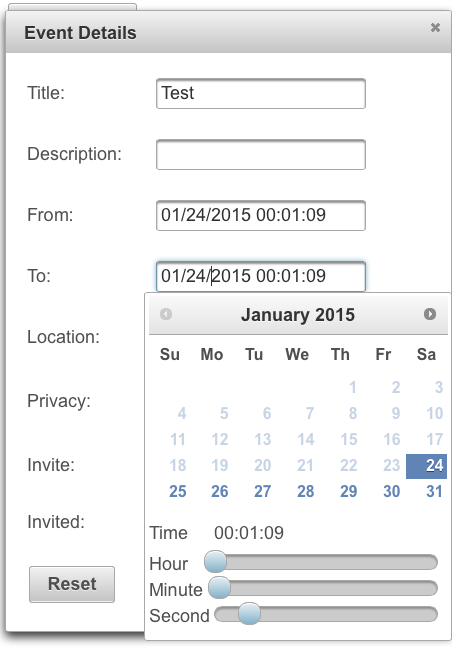
\includegraphics[width=0.7\linewidth]{./images/10_date_select.png}
\end{center}

Places and users have to be selected from the autocomplete.
In order to search for a place you have to specify its name. The system will let you choose 
between the different cities with the same name.
In order to search for a user you have to specify its username. The system will provide results showing users email (which are the unique user id). You then have to choose the email of the user you want to invite. 

After the first invite is sent the form is updated. You can see an updated list of the user you have invited right under the “invite user autocomplete”. You can invite as many people as you want before saving.

The following three picture show: 
\begin{enumerate}
\item A place selection with two alternatives.
\item The selection of a user to invite him
\item The updated form after the invite is sent
\end{enumerate}

\begin{center}
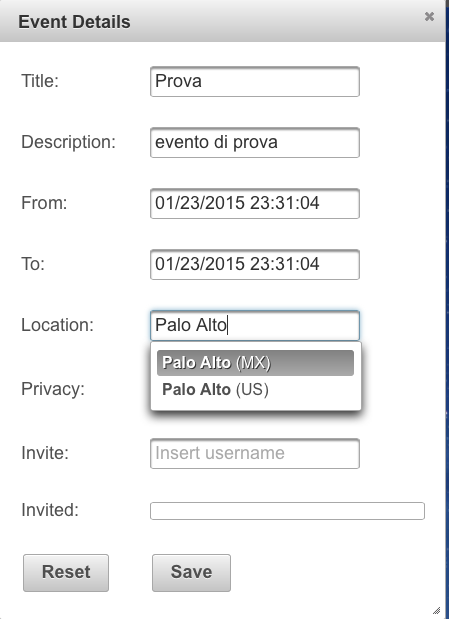
\includegraphics[width=0.5\linewidth]{./images/11_choose_place.png}
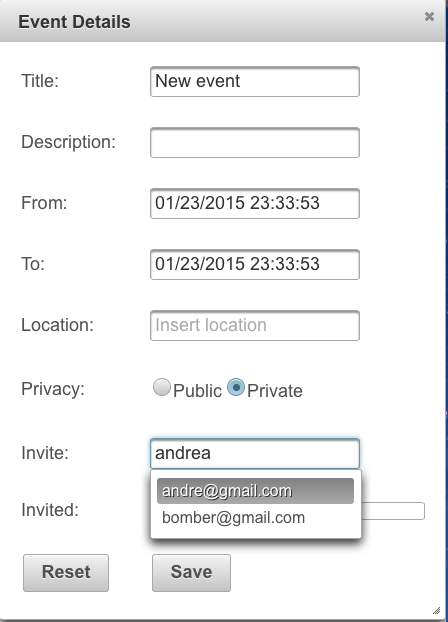
\includegraphics[width=0.5\linewidth]{./images/12_invite_user.png}
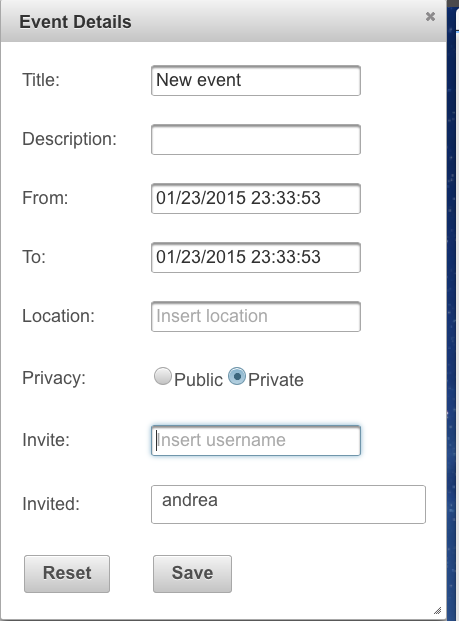
\includegraphics[width=0.5\linewidth]{./images/13_after_invite.png}
\end{center}

\subsection{Check, modify, delete event}
You can check the details of an event by simply clicking on it. A dialog containing all the relevant information will be displayed. For example:

\begin{center}
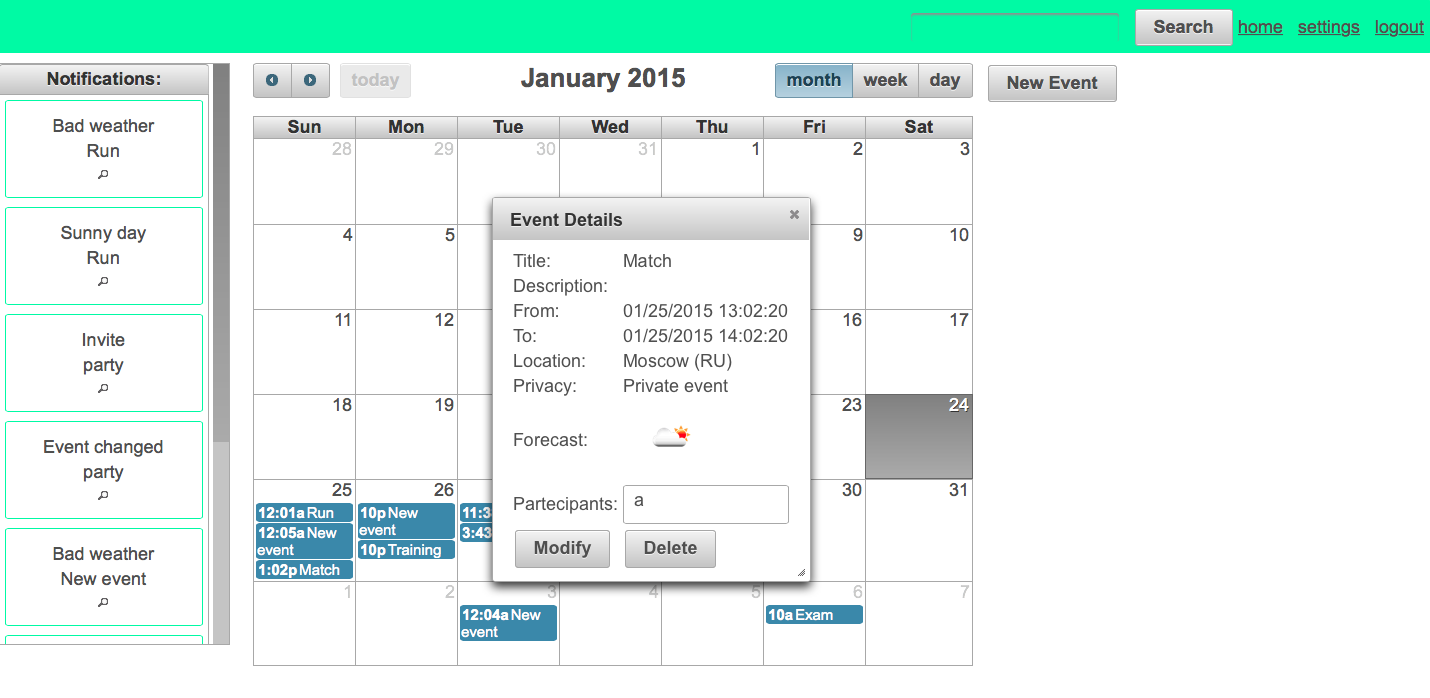
\includegraphics[width=\linewidth]{./images/14_home_details.png}
\end{center}

The details dialog allows the creator of the event to delete (the event is deleted for all its participants) or modify the event.

“Modify Event” will open the dialog on the right of the calendar where you can update event details. Note that the dialog displays the updated information of the event you are modifying.

The following images show some of the features of event detail dialogs for event creator.

\begin{center}
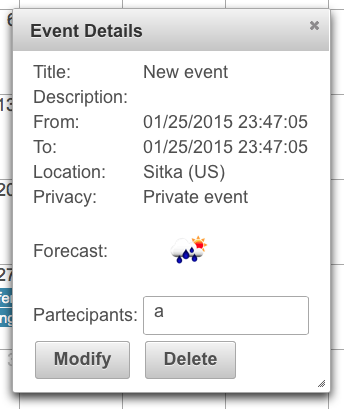
\includegraphics[width=0.5\linewidth]{./images/15_creator_details_1}
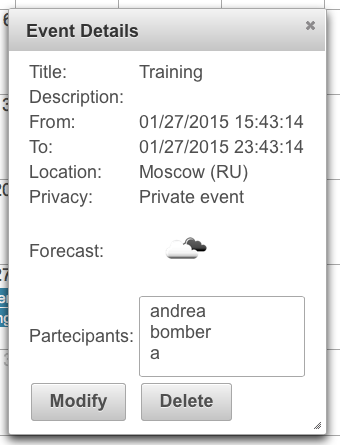
\includegraphics[width=0.5\linewidth]{./images/16_creator_details_2}
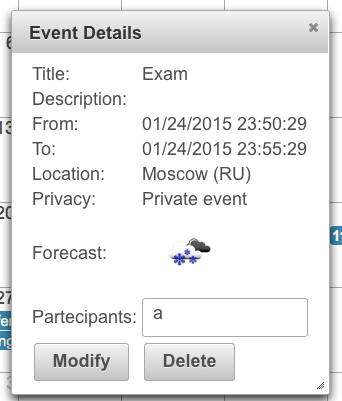
\includegraphics[width=0.5\linewidth]{./images/17_creator_details_3}
\end{center}

A participant (an invited user) is able to see event details but can’t modify or delete it. A participant can only decide to remove his unregister for the selected event, removing himself/herself from the list of participants.

\begin{center}
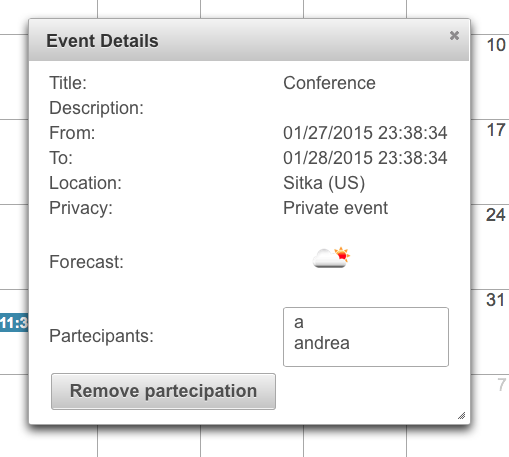
\includegraphics[width=0.7\linewidth]{./images/18_details_partecipant}
\end{center}


\section{Search}

\subsection{Search}
Using the top bar you can search for other users. The search key might be the username, the name or the user’s surname. Results are shown in the result page. The following image shows the results corresponding to the search key “andrea”.

\begin{center}
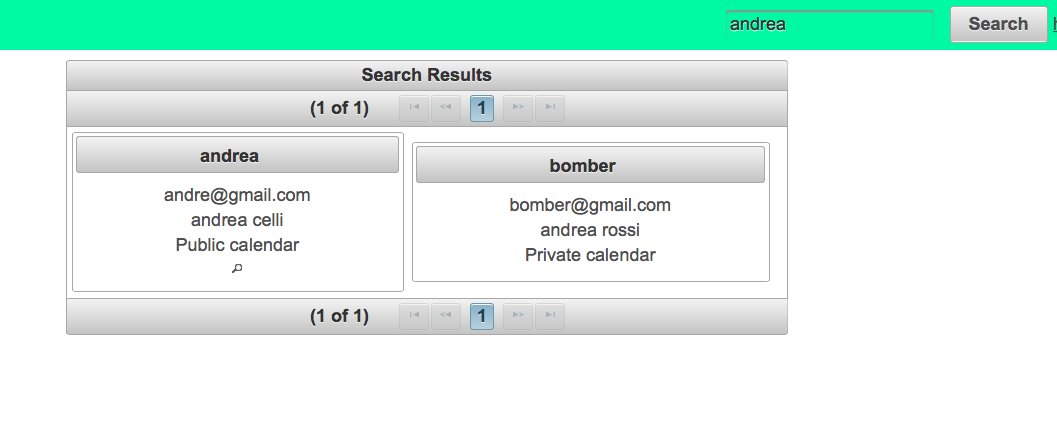
\includegraphics[width=0.7\linewidth]{./images/19_search_results}
\end{center}

In more detail:

\begin{center}
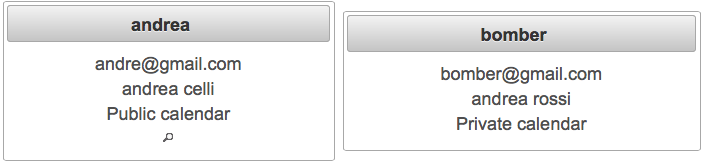
\includegraphics[width=0.7\linewidth]{./images/20_search_results_detail}
\end{center}

\subsection{View other user page}
Andrea Celli has a public calendar. You can go to his calendar by clicking on the lens. Andrea Rossi has a private calendar. Therefore you can’t browse his calendar page. If you have clicked the lens to Andrea Celli’s calendar you’ll be redirected to a page showing his calendar.

This is an example of a search that didn’t find any result.

\begin{center}
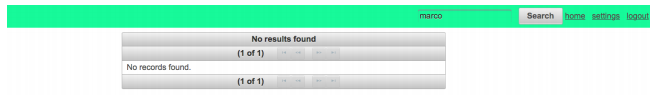
\includegraphics[width=\linewidth]{./images/21_search_no_results}
\end{center}

The following image shows an example of another user’s calendar.

\begin{center}
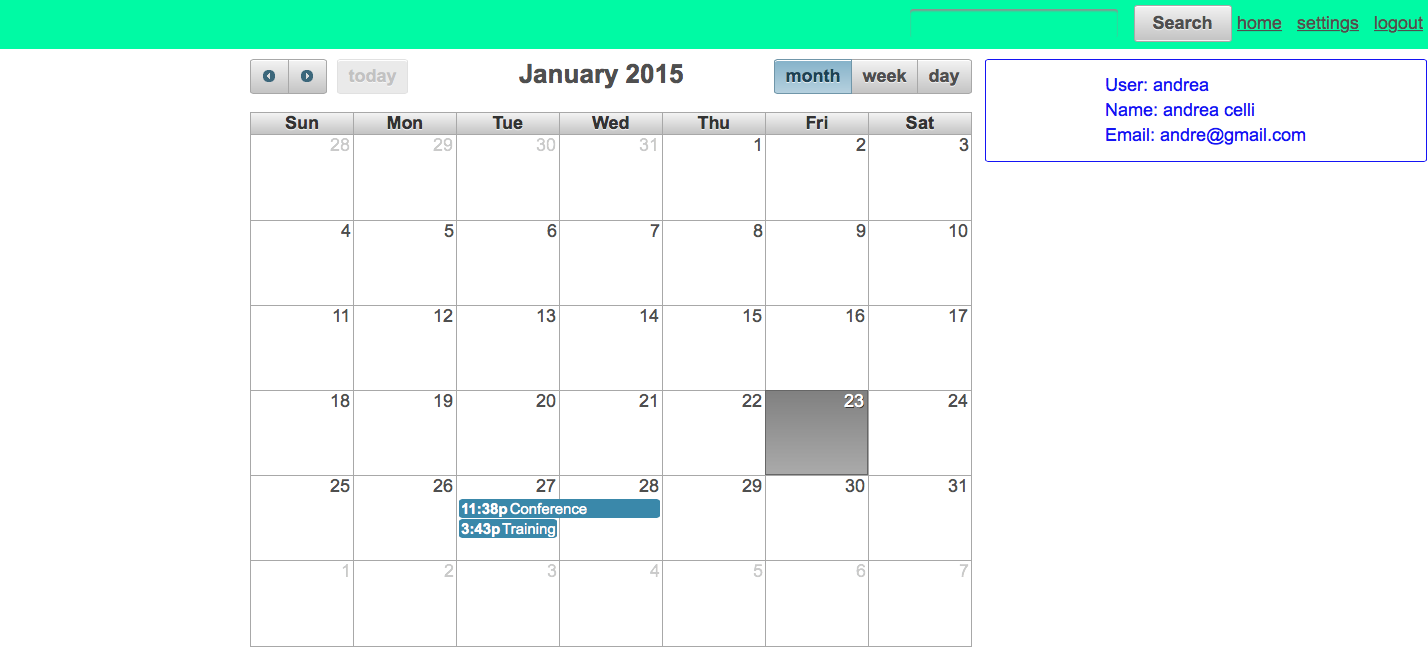
\includegraphics[width=\linewidth]{./images/22_other_user_page}
\end{center}

On the right you can see the details of the selected user.
When you click on one of the displayed events the system will check whether the event is public or private.
In case of public event the details (title, description, start/end, location) will be displayed in a dialog.
Otherwise, if the event is private, you will be able to see only the starting time/date and the ending time/date of the event. 

The following image gives an example of the details of a private event.

\begin{center}
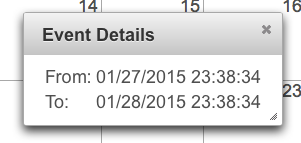
\includegraphics[width=0.7\linewidth]{./images/23_event_details_private}
\end{center}

\section{Notifications}
You can receive different type of notifications. You will find all of them on the left, in the notifications panel. If the number of notifications is high you will be able to scroll the panel.

In this picture the user is scrolling his notifications.

\begin{center}
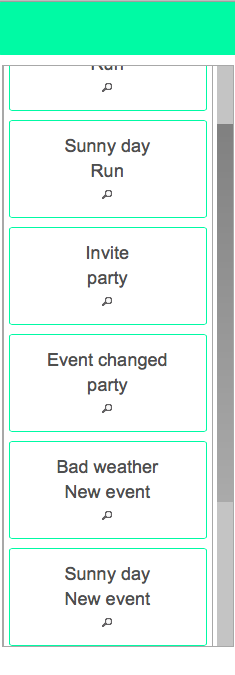
\includegraphics[width=0.3\linewidth]{./images/24_notification_scroll}
\end{center}

You can read a notification by clicking on the lens under the title of the referred event. When you click on it the system displays a dialog that shows details about the notification and asks for your response.

In case of bad weather alert and event changed notification you can only mark the notification as red using the OK button. The same situation arises when the system is not able to find a sunny day for a “sunny day proposal”. 

In case of invites and sunny day proposals you are asked whether to accept or decline. You can answer using “Accept” and “Decline” button. When you close a notification dialog without explicitly answering the notification is not marked as red, therefore it will still be in your notification panel.

The following images show all the different types of notifications.

\begin{center}
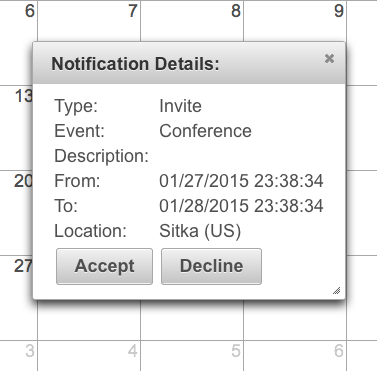
\includegraphics[width=0.7\linewidth]{./images/25_notification_invite}\vspace{10pt}
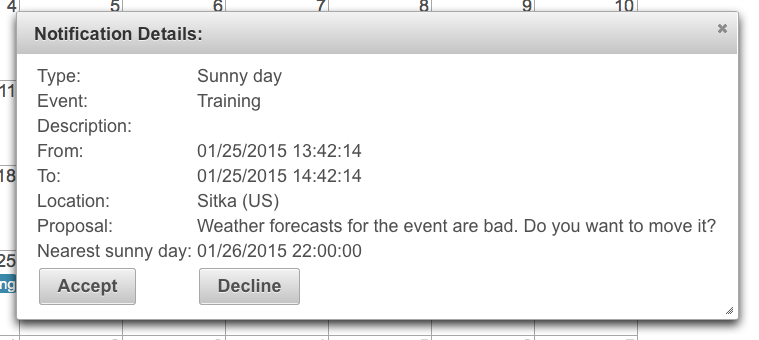
\includegraphics[width=0.7\linewidth]{./images/26_sunny_day_proposal}\vspace{10pt}
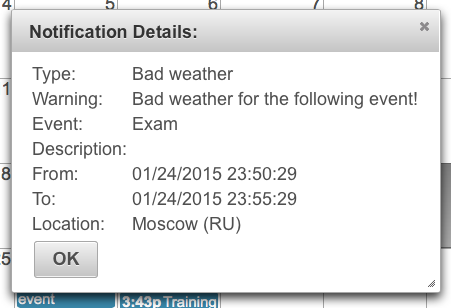
\includegraphics[width=0.7\linewidth]{./images/27_bad_weather_alert}\vspace{10pt}
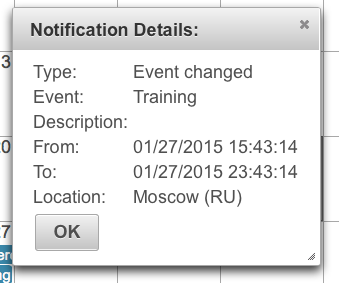
\includegraphics[width=0.7\linewidth]{./images/28_event_changed_notification}
\end{center}

\section{Settings}
You can change your personal details using your settings page. You can input new personal data into the forms. You can’t save leaving any of them blank. This is an example of a settings page.

\begin{center}
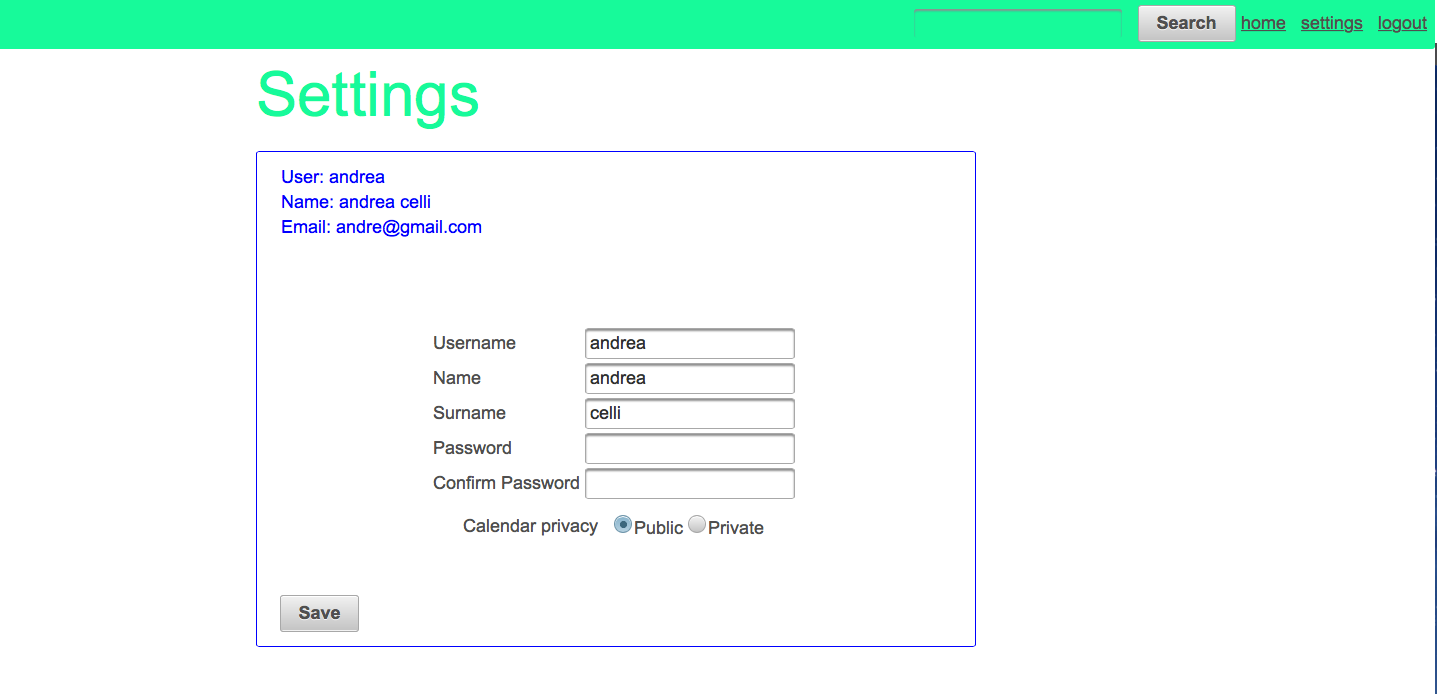
\includegraphics[width=\linewidth]{./images/29_settings}
\end{center}

\part{Errors}
When managing your personal data (login, registration, settings) errors may occur. The following images gives an idea of the way in which error are displayed.

\section{Login errors}
\begin{center}
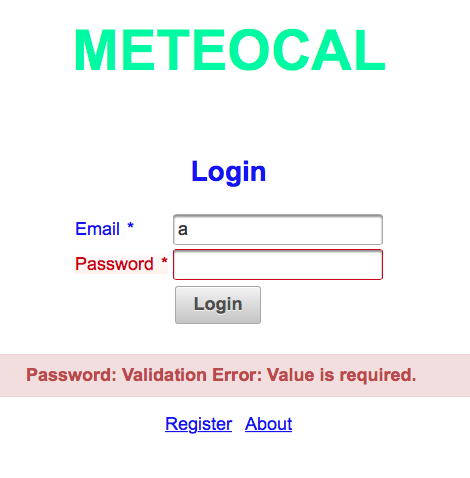
\includegraphics[width=0.7\linewidth]{./images/30_error_login_1}
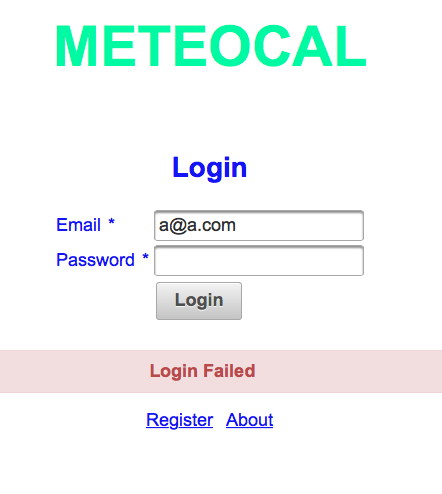
\includegraphics[width=0.7\linewidth]{./images/31_error_login_2}
\end{center}

\section{Registration errors}
\begin{center}
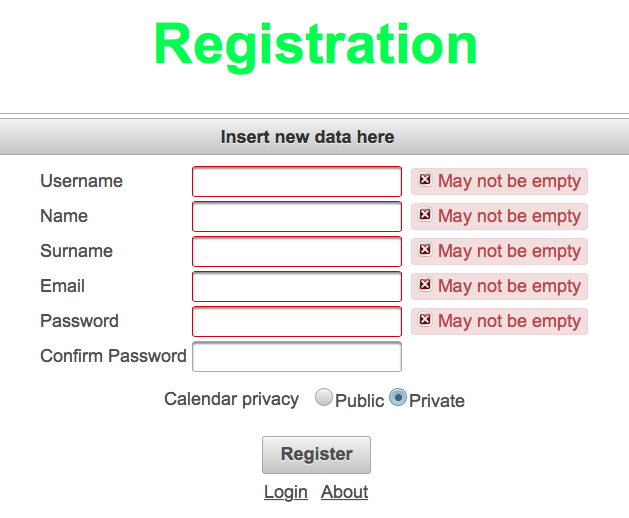
\includegraphics[width=0.7\linewidth]{./images/32_error_registration_1}
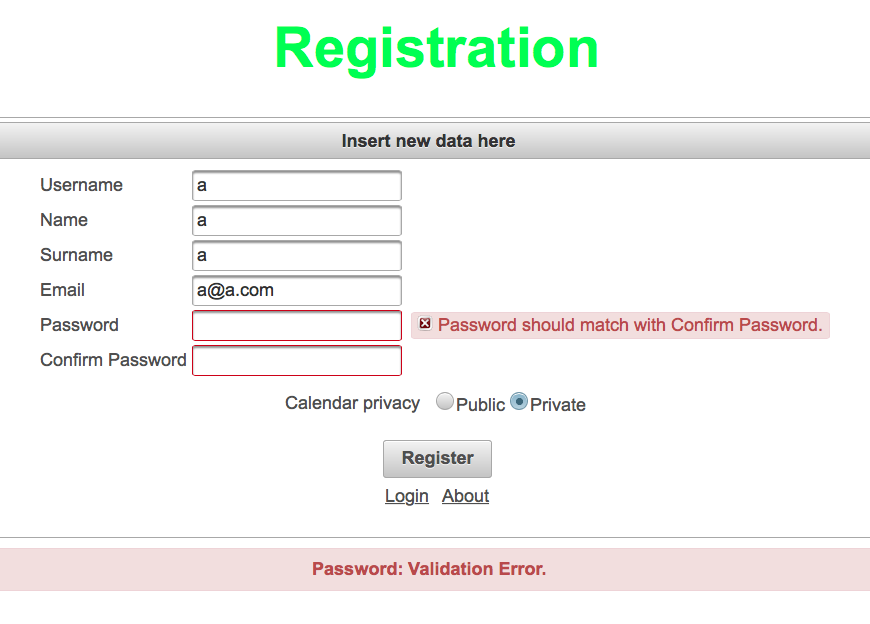
\includegraphics[width=0.7\linewidth]{./images/33_error_registration_2}
\end{center}

\section{Settings error}
\begin{center}
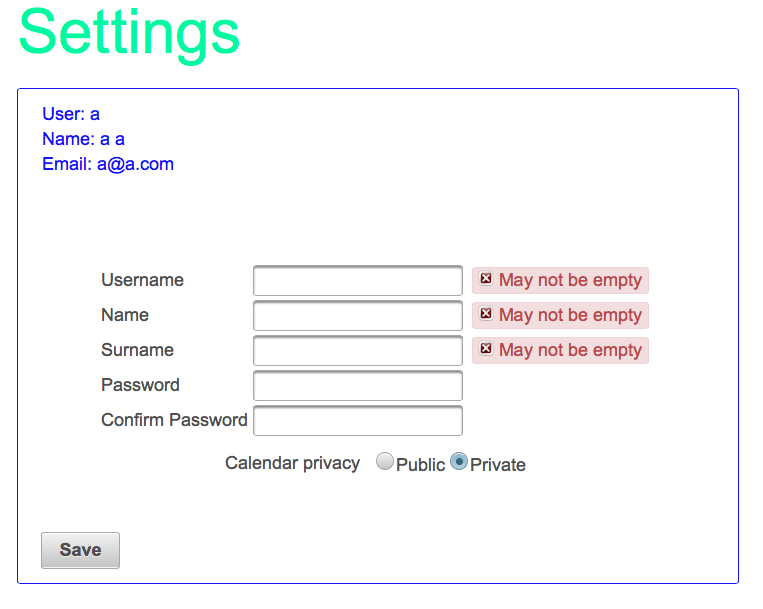
\includegraphics[width=0.7\linewidth]{./images/34_error_settings_1}
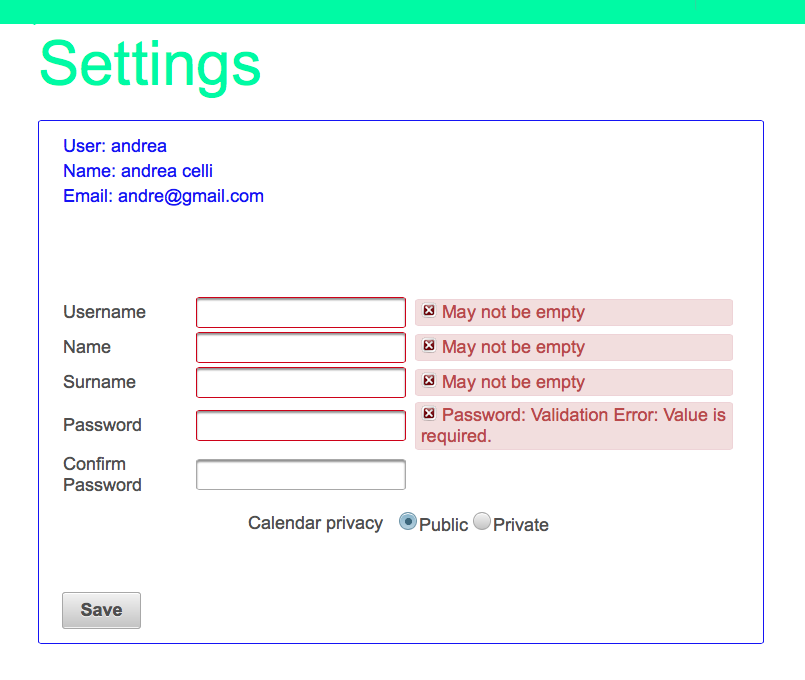
\includegraphics[width=0.7\linewidth]{./images/35_error_settings_2}
\end{center}

\end{document}